% !TEX program = xelatex
% ============================================================================
% Diagrama Entidad-Relacion (notacion de Chen extendida con AGREGACIONES)
% Proyecto Final Bases de Datos - Inventario, Compras y Ventas (PostgreSQL)
% Sincronizado con Scripts sql/ - Tipografia Source Sans 3 + JetBrains Mono
%
% RELACIONES M:N (tabla puente, rombo + atributos):
%   suministra  → producto_proveedor
%   solicita    → detalle_orden_compra      (Agregacion A1)
%   recibe      → detalle_recepcion         (sobre Agregacion A1)
%   mantiene    → inventarios               (Agregacion A2)
%   traslada    → detalle_transferencia     (sobre Agregacion A2)
%   contiene    → detalle_pedido            (Agregacion A3)
%   devuelve    → detalle_devolucion        (sobre Agregacion A3)
%
% RELACIONES 1:N / 1:1 (FK directa, linea simple con cardinalidades):
%   sedes 1 ─── N almacenes
%   sedes 1 ─── N empleados
%   categorias 1 ─── N productos
%   empleados 1 ─── 1 usuarios
%   usuarios 1 ─── N auditoria_accesos
%   proveedores 1 ─── N ordenes_compra
%   almacenes 1 ─── N ordenes_compra (almacen_destino)
%   empleados 1 ─── N ordenes_compra
%   ordenes_compra 1 ─── N recepciones_compra
%   almacenes 1 ─── N transferencias (origen)
%   almacenes 1 ─── N transferencias (destino)
%   sedes 1 ─── N pedidos_venta
%   almacenes 1 ─── N pedidos_venta
%   clientes 1 ─── N pedidos_venta
%   empleados 1 ─── N pedidos_venta
%   pedidos_venta 1 ─── N devoluciones
%   pedidos_venta 1 ─── N pagos
% ============================================================================
\documentclass[tikz, border=28pt]{standalone}

\usepackage{fontspec}
\IfFontExistsTF{SourceSans3-Regular}{%
  \setmainfont{SourceSans3-Regular}[
    BoldFont = SourceSans3-Bold,
    ItalicFont = SourceSans3-It,
    BoldItalicFont = SourceSans3-BoldIt
  ]%
  \setsansfont{SourceSans3-Regular}[
    BoldFont = SourceSans3-Bold,
    ItalicFont = SourceSans3-It,
    BoldItalicFont = SourceSans3-BoldIt
  ]%
}{%
  \setmainfont{Source Sans 3}%
  \setsansfont{Source Sans 3}%
}
\IfFontExistsTF{JetBrainsMono-Regular}{%
  \setmonofont{JetBrainsMono-Regular}[
    Scale=0.86,
    BoldFont = JetBrainsMono-Bold,
    ItalicFont = JetBrainsMono-Italic
  ]%
}{%
  \setmonofont{JetBrains Mono}[Scale=0.86]%
}

\usetikzlibrary{
  shapes.geometric, shapes.multipart,
  calc, shadows, fit, backgrounds
}

% ----------------------------------------------------------------
% CAPAS
% ----------------------------------------------------------------
\pgfdeclarelayer{zonas}
\pgfdeclarelayer{agr}
\pgfsetlayers{zonas,agr,main}

% ----------------------------------------------------------------
% PALETA DE COLORES
% ----------------------------------------------------------------
\definecolor{cCat}{HTML}{1A5DA8}   % catalogo_terceros          — azul
\definecolor{cCom}{HTML}{C96800}   % compras_abastecimiento     — naranja
\definecolor{cInv}{HTML}{1E7A45}   % inventarios_transferencias — verde
\definecolor{cVen}{HTML}{A82010}   % ventas_pagos               — rojo
\definecolor{cIde}{HTML}{6030A0}   % identidad_accesos          — purpura
\definecolor{cRep}{HTML}{2C3E50}   % reportes                   — gris azul

\definecolor{relFill}{HTML}{FFFAE8}
\definecolor{relBorder}{HTML}{B8A010}
\definecolor{attFill}{HTML}{FAFAFA}
\definecolor{bgCanvas}{HTML}{F6F8FB}

% ----------------------------------------------------------------
% ESTILOS
% ----------------------------------------------------------------
\tikzset{
  %% ---- entidades (rectangle split bipartito) ----
  ent/.style={
    draw=black!65, line width=1.4pt,
    rectangle split, rectangle split parts=2,
    font=\sffamily\fontsize{13.5}{17.2}\selectfont,
    align=left, inner sep=7pt, text width=6.6cm,
    drop shadow={shadow xshift=2pt, shadow yshift=-2pt,
                 fill=black!20, opacity=0.32}
  },
  entC/.style={ent,
    draw=cCat!75!black,
    rectangle split part fill={cCat!26!white, cCat!5!white}},
  entK/.style={ent,
    draw=cCom!75!black,
    rectangle split part fill={cCom!28!white, cCom!6!white}},
  entI/.style={ent,
    draw=cInv!75!black,
    rectangle split part fill={cInv!26!white, cInv!5!white}},
  entV/.style={ent,
    draw=cVen!75!black,
    rectangle split part fill={cVen!26!white, cVen!5!white}},
  entU/.style={ent,
    draw=cIde!75!black,
    rectangle split part fill={cIde!26!white, cIde!5!white}},
  %% ---- relaciones M:N (rombos) ----
  rel/.style={
    draw=relBorder, line width=1.4pt,
    diamond, aspect=2.1,
    font=\sffamily\bfseries\fontsize{12.8}{14.8}\selectfont,
    align=center, inner sep=1pt,
    minimum width=3.8cm, minimum height=1.9cm,
    fill=relFill
  },
  %% ---- atributos ----
  att/.style={
    draw=black!55, line width=1.0pt,
    ellipse, fill=attFill,
    font=\sffamily\fontsize{12}{14}\selectfont,
    inner sep=4pt, minimum height=0.95cm
  },
  datt/.style={att, densely dashed, draw=black!48},
  %% ---- cardinalidades sobre lineas ----
  card/.style={
    font=\sffamily\bfseries\fontsize{13.5}{15.5}\selectfont,
    fill=white, inner sep=2.5pt, rounded corners=2pt,
    text=black!85
  },
  %% ---- lineas ----
  fisica/.style={line width=1.4pt, black!82},
  logica/.style={line width=1.4pt, densely dashed, black!55},
  aline/.style={line width=0.95pt, black!48},
  %% ---- zonas de microservicio / esquema ----
  zone/.style={
    rounded corners=12pt,
    draw=#1!42, fill=#1!4.5!bgCanvas,
    line width=1.25pt,
    inner sep=26pt
  },
  ztab/.style={
    font=\sffamily\bfseries\fontsize{13}{16}\selectfont,
    text=white, fill=#1!78!black,
    rounded corners=4pt, inner sep=6pt,
    anchor=south west
  },
  ztabR/.style={
    ztab=#1,
    anchor=south east
  },
  %% ---- cajas de agregacion EER (entidades + relacion M:N) ----
  agr/.style={
    draw=#1!85!black, line width=2.0pt,
    dash pattern=on 8pt off 4pt,
    rounded corners=9pt,
    fill=none
  },
  agrtab/.style={
    font=\sffamily\bfseries\fontsize{11.8}{13.8}\selectfont,
    text=#1!80!black, fill=white, rounded corners=3pt,
    anchor=south west, inner sep=3.5pt
  },
  agrtabR/.style={
    agrtab=#1,
    anchor=south east
  }
}

% ----------------------------------------------------------------
% MACROS
% ----------------------------------------------------------------
\newcommand{\pk}[1]{\underline{\textbf{#1}}}
\newcommand{\fk}{\textsuperscript{\fontsize{8.5}{10}\selectfont\sffamily\bfseries\ FK}}
\newcommand{\uq}{\textsuperscript{\fontsize{8.5}{10}\selectfont\sffamily\bfseries\ U}}

% \entity{estilo}{id}{pos}{esquema}{nombre}{atributos}
\newcommand{\entity}[6]{%
  \node[#1] (#2) at (#3)
  {{\centering
     {\fontsize{10}{11.5}\selectfont\color{black!60}\ttfamily\bfseries #4.}\\[1pt]
     {\fontsize{16}{19}\selectfont\bfseries #5}\par}%
   \nodepart{second}#6};}

% \zone{color}{id}{etiqueta}{fit-list}
\newcommand{\zone}[4]{%
  \begin{pgfonlayer}{zonas}
    \node[zone=#1, fit=#4] (#2) {};
    \node[ztab=#1] at ([xshift=14pt]#2.north west) {#3};
  \end{pgfonlayer}}

% Variante con etiqueta alineada a la esquina superior derecha
\newcommand{\zoneR}[4]{%
  \begin{pgfonlayer}{zonas}
    \node[zone=#1, fit=#4] (#2) {};
    \node[ztabR=#1] at ([xshift=-14pt]#2.north east) {#3};
  \end{pgfonlayer}}

% ----------------------------------------------------------------
\begin{document}
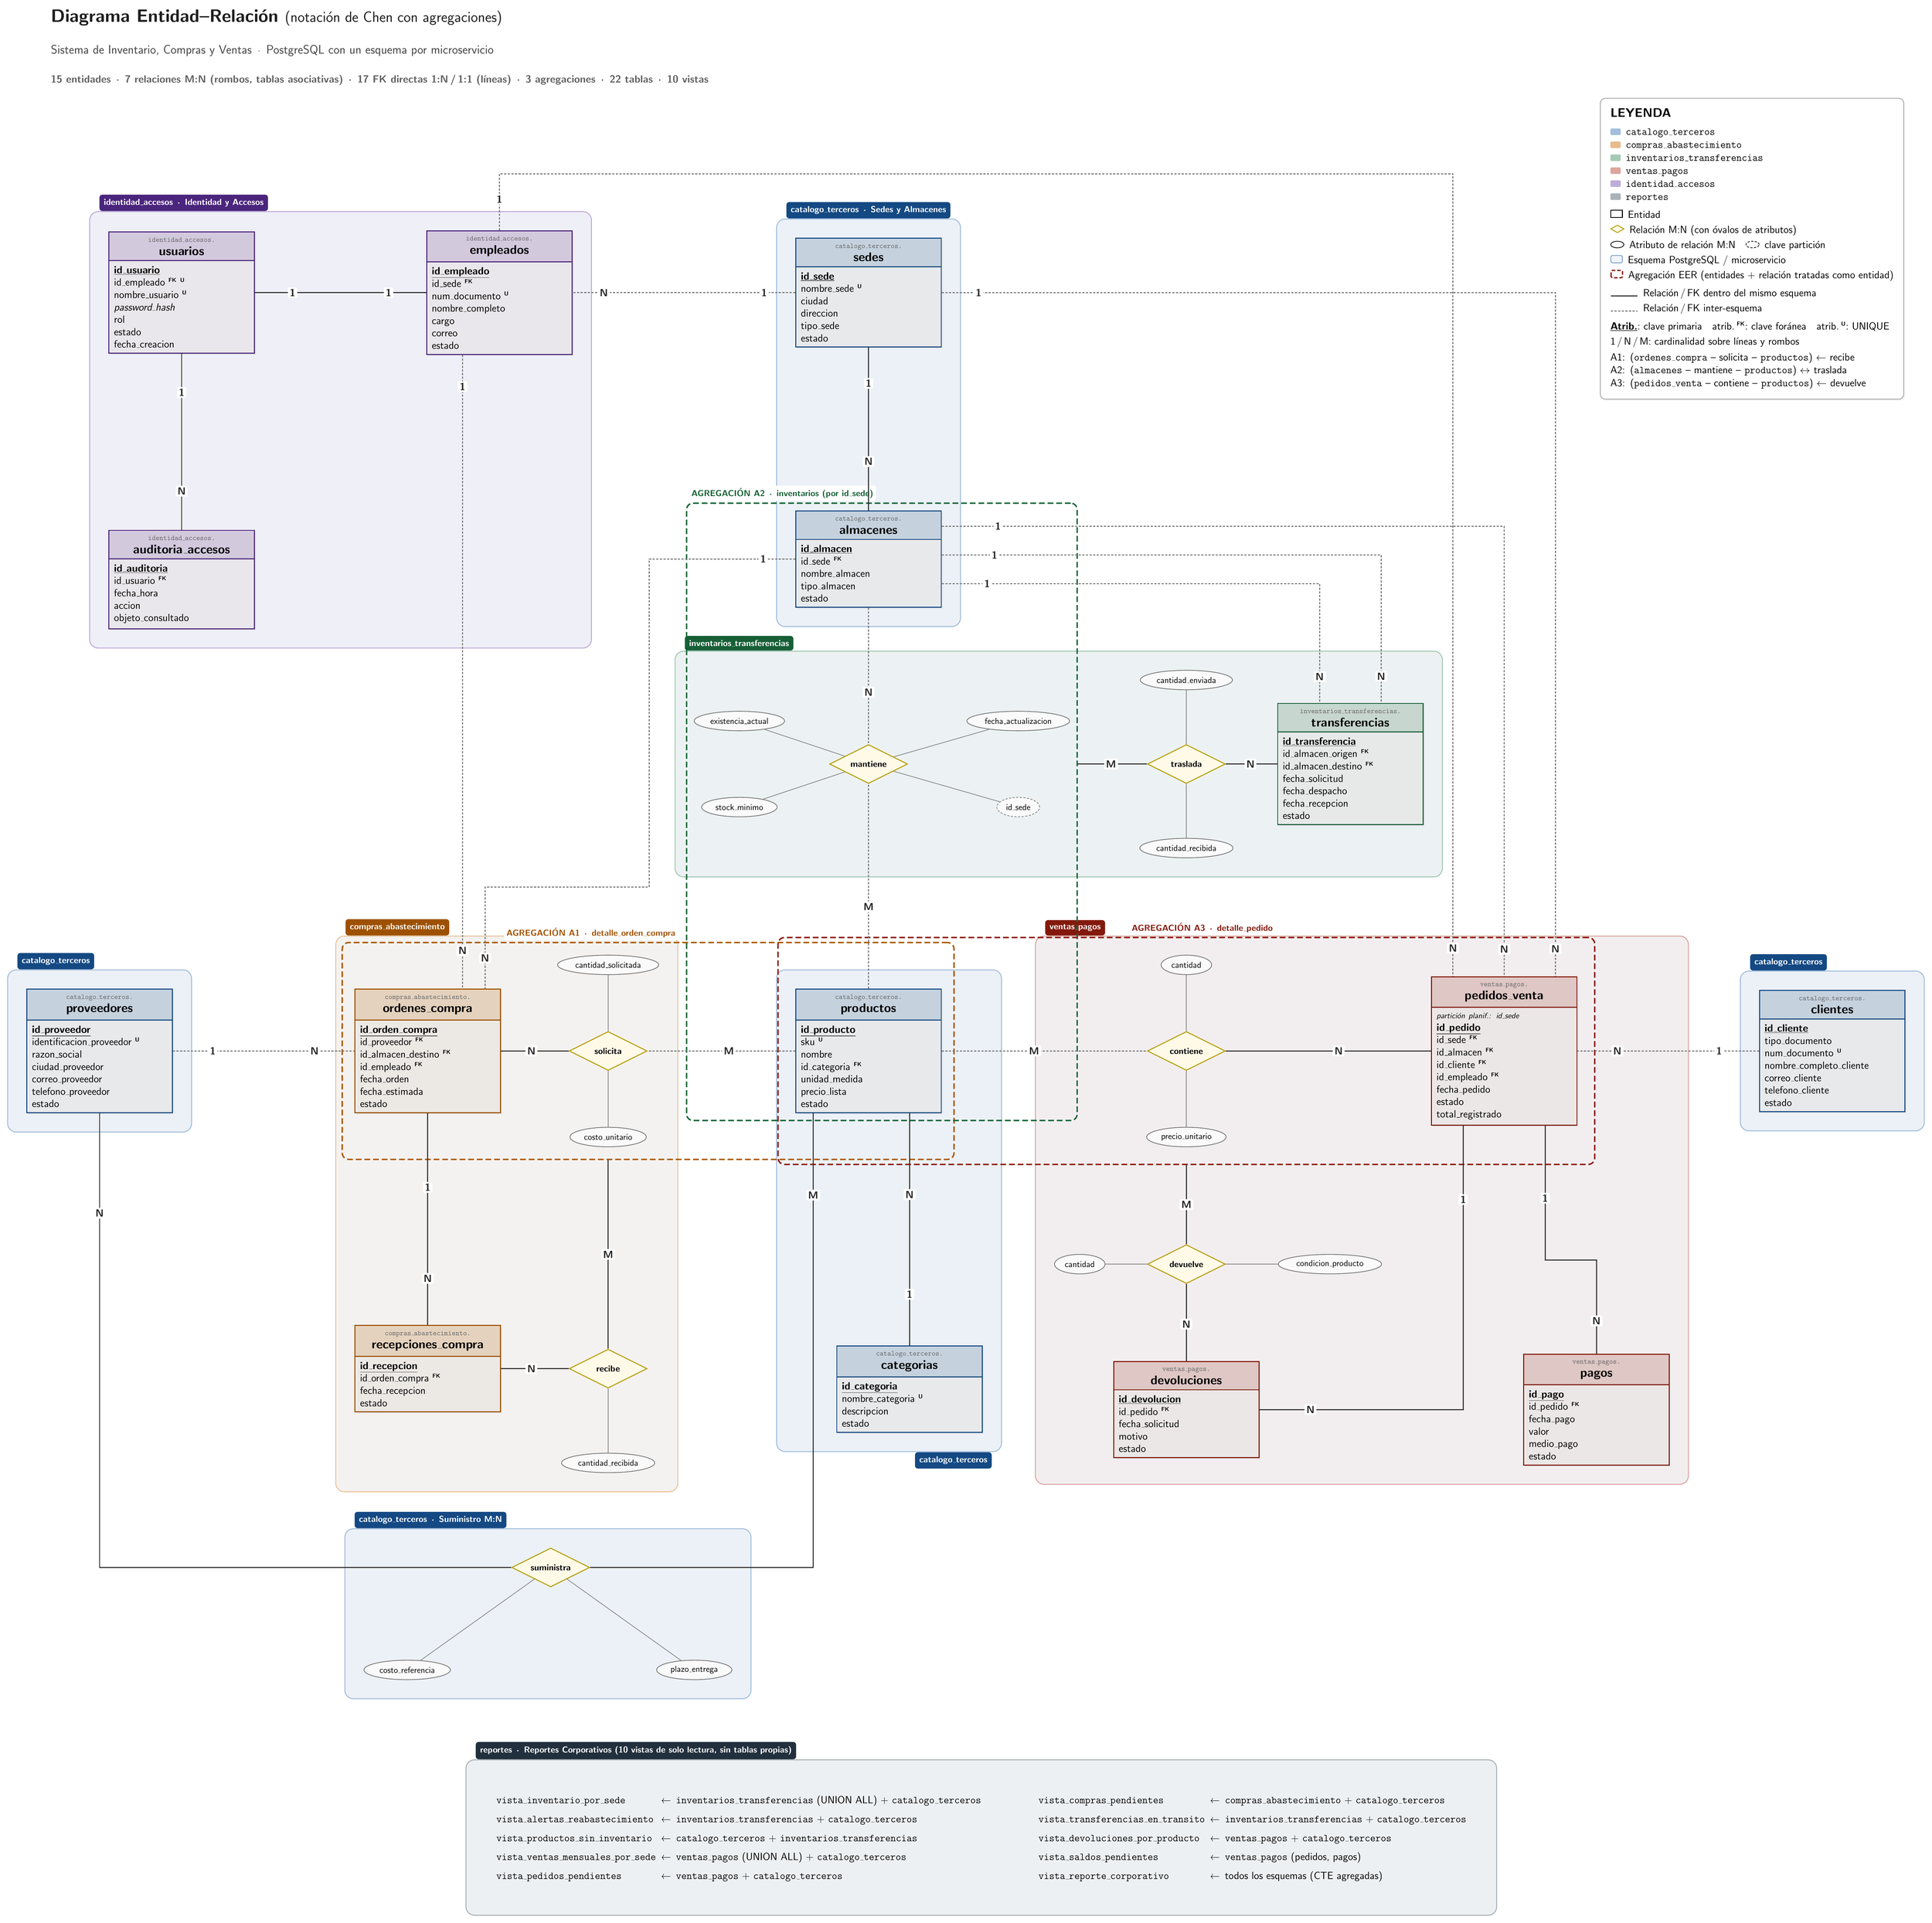
\begin{tikzpicture}

% ====================================================================
% ENTIDADES
% ====================================================================

% ---- identidad_accesos ----
\entity{entU}{usu}{0,0}{identidad\_accesos}{usuarios}
  {\pk{id\_usuario}\\id\_empleado\fk\uq\\nombre\_usuario\uq\\\textit{password\_hash}\\rol\\estado\\fecha\_creacion}

\entity{entU}{emp}{15.5,0}{identidad\_accesos}{empleados}
  {\pk{id\_empleado}\\id\_sede\fk\\num\_documento\uq\\nombre\_completo\\cargo\\correo\\estado}

\entity{entU}{aud}{0,-14.0}{identidad\_accesos}{auditoria\_accesos}
  {\pk{id\_auditoria}\\id\_usuario\fk\\fecha\_hora\\accion\\objeto\_consultado}

% ---- catalogo_terceros ----
\entity{entC}{sed}{33.5,0}{catalogo\_terceros}{sedes}
  {\pk{id\_sede}\\nombre\_sede\uq\\ciudad\\direccion\\tipo\_sede\\estado}

\entity{entC}{alm}{33.5,-13.0}{catalogo\_terceros}{almacenes}
  {\pk{id\_almacen}\\id\_sede\fk\\nombre\_almacen\\tipo\_almacen\\estado}

\entity{entC}{pro}{33.5,-37.0}{catalogo\_terceros}{productos}
  {\pk{id\_producto}\\sku\uq\\nombre\\id\_categoria\fk\\unidad\_medida\\precio\_lista\\estado}

\entity{entC}{cat}{35.5,-53.5}{catalogo\_terceros}{categorias}
  {\pk{id\_categoria}\\nombre\_categoria\uq\\descripcion\\estado}

\entity{entC}{prv}{-4.0,-37.0}{catalogo\_terceros}{proveedores}
  {\pk{id\_proveedor}\\identificacion\_proveedor\uq\\razon\_social\\ciudad\_proveedor\\correo\_proveedor\\telefono\_proveedor\\estado}

\entity{entC}{cli}{80.5,-37.0}{catalogo\_terceros}{clientes}
  {\pk{id\_cliente}\\tipo\_documento\\num\_documento\uq\\nombre\_completo\_cliente\\correo\_cliente\\telefono\_cliente\\estado}

% ---- compras_abastecimiento ----
\entity{entK}{oc}{12.0,-37.0}{compras\_abastecimiento}{ordenes\_compra}
  {\pk{id\_orden\_compra}\\id\_proveedor\fk\\id\_almacen\_destino\fk\\id\_empleado\fk\\fecha\_orden\\fecha\_estimada\\estado}

\entity{entK}{rc}{12.0,-52.5}{compras\_abastecimiento}{recepciones\_compra}
  {\pk{id\_recepcion}\\id\_orden\_compra\fk\\fecha\_recepcion\\estado}

% ---- inventarios_transferencias ----
\entity{entI}{tr}{57.0,-23.0}{inventarios\_transferencias}{transferencias}
  {\pk{id\_transferencia}\\id\_almacen\_origen\fk\\id\_almacen\_destino\fk\\fecha\_solicitud\\fecha\_despacho\\fecha\_recepcion\\estado}

% ---- ventas_pagos ----
\entity{entV}{pv}{64.5,-37.0}{ventas\_pagos}{pedidos\_venta}
  {\textit{\fontsize{10.5}{12.5}\selectfont partici\'on planif.: id\_sede}\\
   \pk{id\_pedido}\\id\_sede\fk\\id\_almacen\fk\\id\_cliente\fk\\id\_empleado\fk\\fecha\_pedido\\estado\\total\_registrado}

\entity{entV}{dev}{49.0,-54.5}{ventas\_pagos}{devoluciones}
  {\pk{id\_devolucion}\\id\_pedido\fk\\fecha\_solicitud\\motivo\\estado}

\entity{entV}{pag}{69.0,-54.5}{ventas\_pagos}{pagos}
  {\pk{id\_pago}\\id\_pedido\fk\\fecha\_pago\\valor\\medio\_pago\\estado}

% ====================================================================
% RELACIONES M:N (ROMBOS con atributos)
% ====================================================================

% suministra: proveedores M:N productos → producto_proveedor
\node[rel] (suministra) at (18.0,-62.2) {suministra};
\node[att] (s1) at (11.0,-67.2) {costo\_referencia};
\node[att] (s2) at (25.0,-67.2) {plazo\_entrega};

% solicita (A1): ordenes_compra M:N productos → detalle_orden_compra
\node[rel] (solicita) at (20.8,-37.0) {solicita};
\node[att] (a11) at (20.8,-32.8) {cantidad\_solicitada};
\node[att] (a12) at (20.8,-41.2) {costo\_unitario};

% recibe: recepciones_compra M:N A1 (ordenes_compra + solicita + productos)
\node[rel] (recibe) at (20.8,-52.5) {recibe};
\node[att] (a13) at (20.8,-57.1) {cantidad\_recibida};

% mantiene (A2): almacenes M:N productos → inventarios
\node[rel] (mantiene) at (33.5,-23.0) {mantiene};
\node[att]  (b1) at (27.2,-20.9) {existencia\_actual};
\node[att]  (b2) at (27.2,-25.1) {stock\_minimo};
\node[att]  (b3) at (40.8,-20.9) {fecha\_actualizacion};
\node[datt] (b4) at (40.8,-25.1) {id\_sede};

% traslada: A2 (almacenes + mantiene + productos) M:N transferencias
\node[rel] (traslada) at (49.0,-23.0) {traslada};
\node[att] (c1) at (49.0,-18.9) {cantidad\_enviada};
\node[att] (c2) at (49.0,-27.1) {cantidad\_recibida};

% contiene (A3): pedidos_venta M:N productos → detalle_pedido
\node[rel] (contiene) at (49.0,-37.0) {contiene};
\node[att] (d1) at (49.0,-32.8) {cantidad};
\node[att] (d2) at (49.0,-41.2) {precio\_unitario};

% devuelve: devoluciones M:N A3 (pedidos_venta + contiene + productos)
\node[rel] (devuelve) at (49.0,-47.4) {devuelve};
\node[att] (e1) at (43.8,-47.4) {cantidad};
\node[att] (e2) at (56.0,-47.4) {condicion\_producto};

% ====================================================================
% CAJAS DE AGREGACION EER (entidades + relacion M:N tratadas como entidad)
% ====================================================================
\begin{pgfonlayer}{agr}
  % A1: ordenes_compra + solicita + productos -> detalle_orden_compra
  \node[agr=cCom, inner sep=17pt, fit=(oc)(solicita)(a11)(a12)(pro)] (A1) {};
  \node[agrtab=cCom, anchor=south west] (A1lab) at ([xshift=6pt,yshift=2pt]15.5,-31.67)
    {AGREGACI\'ON A1\enspace·\enspace detalle\_orden\_compra};

  % A2: almacenes + mantiene + productos -> inventarios
  \node[agr=cInv, inner sep=10pt, fit=(alm)(mantiene)(b1)(b2)(b3)(b4)(pro)] (A2) {};
  \node[agrtab=cInv, anchor=south west] (A2lab) at ([xshift=4pt,yshift=2pt]A2.north west)
    {AGREGACI\'ON A2\enspace·\enspace inventarios (por id\_sede)};

  % A3: pedidos_venta + contiene + productos -> detalle_pedido
  \node[agr=cVen, inner sep=24pt, fit=(pro)(contiene)(d1)(d2)(pv)] (A3) {};
  \node[agrtab=cVen, anchor=south] (A3lab) at ([xshift=22pt,yshift=2pt]A3.north -| contiene)
    {AGREGACI\'ON A3\enspace·\enspace detalle\_pedido};
\end{pgfonlayer}

% ====================================================================
% LINEAS DE ATRIBUTO (aline: fina, hacia su rombo)
% ====================================================================
\foreach \a/\r in {
  s1/suministra, s2/suministra,
  a11/solicita,  a12/solicita,  a13/recibe,
  b1/mantiene,   b2/mantiene,   b3/mantiene, b4/mantiene,
  c1/traslada,   c2/traslada,
  d1/contiene,   d2/contiene,
  e1/devuelve,   e2/devuelve}
  \draw[aline] (\a) -- (\r);

% ====================================================================
% RELACIONES M:N — lineas desde/hacia rombos y agregaciones
% ====================================================================

% suministra: proveedores ─N─ suministra ─M─ productos
\draw[fisica] (prv.south) -- node[card,pos=.22]{N} (-4.0,-62.2) -- (suministra.west);
\draw[fisica] (suministra.east) -- (30.8,-62.2) -- node[card,pos=.82]{M} ($(pro.south)+(-2.7,0)$);

% solicita (A1): ordenes_compra ─N─ solicita ─M─ productos
\draw[fisica] (oc.east)  -- node[card,pos=.45]{N} (solicita.west);
\draw[logica] (pro.west) -- node[card,pos=.45]{M} (solicita.east);

% recibe: recepciones_compra ─N─ recibe ─M─ A1 (detalle_orden_compra)
\draw[fisica] (rc.east)      -- node[card,pos=.45]{N} (recibe.west);
\draw[fisica] (recibe.north) -- node[card,pos=.5]{M}  (recibe.north |- A1.south);

% mantiene (A2): almacenes ─N─ mantiene ─M─ productos
\draw[logica] (alm.south) -- node[card,pos=.62]{N} (mantiene.north);
\draw[logica] (pro.north) -- node[card,pos=.40]{M} (mantiene.south);

% traslada: A2 (inventarios) ─M─ traslada ─N─ transferencias
\draw[fisica] (A2.east |- traslada.west) -- node[card,pos=.48]{M} (traslada.west);
\draw[fisica] (traslada.east)            -- node[card,pos=.48]{N} (tr.west);

% contiene (A3): pedidos_venta ─N─ contiene ─M─ productos
\draw[fisica] (pv.west)  -- node[card,pos=.45]{N} (contiene.east);
\draw[logica] (pro.east) -- node[card,pos=.45]{M} (contiene.west);

% devuelve: devoluciones ─N─ devuelve ─M─ A3 (detalle_pedido)
\draw[fisica] (dev.north)      -- node[card,pos=.48]{N} (devuelve.south);
\draw[fisica] (devuelve.north) -- node[card,pos=.5]{M}  (devuelve.north |- A3.south);

% ====================================================================
% RELACIONES 1:N Y 1:1 (FK directas — lineas simples con cardinalidades)
% ====================================================================

%% identidad_accesos ─────────────────────────────────────────────
% usuarios 1:1 empleados  (usuarios.id_empleado FK, UNIQUE)
\draw[fisica] (usu.east)  -- node[card,pos=.22]{1}
                              node[card,pos=.78]{1} (emp.west);

% usuarios 1:N auditoria_accesos  (auditoria.id_usuario FK)
\draw[fisica] (usu.south) -- node[card,pos=.22]{1}
                              node[card,pos=.78]{N} (aud.north);

%% catalogo_terceros ─────────────────────────────────────────────
% sedes 1:N almacenes  (almacenes.id_sede FK)
\draw[fisica] (sed.south) -- node[card,pos=.22]{1}
                              node[card,pos=.70]{N} (alm.north);

% categorias 1:N productos  (productos.id_categoria FK)
\draw[fisica] (cat.north) -- node[card,pos=.22]{1}
                              node[card,pos=.65]{N} ($(pro.south)+(2.0,0)$);

%% identidad_accesos → catalogo_terceros (inter-esquema, punteada)
% sedes 1:N empleados  (empleados.id_sede FK)
\draw[logica] (sed.west) -- node[card,pos=.14]{1}
                             node[card,pos=.86]{N} (emp.east);

%% compras_abastecimiento ────────────────────────────────────────
% proveedores 1:N ordenes_compra  (ordenes_compra.id_proveedor FK)
\draw[logica] (prv.east) -- node[card,pos=.22]{1}
                             node[card,pos=.78]{N} (oc.west);

% almacenes 1:N ordenes_compra  (ordenes_compra.id_almacen_destino FK)
\draw[logica] (alm.west) -- node[card,pos=.22]{1}
              (22.8,-13.0) -- (22.8,-29.0) -- (14.8,-29.0)
              -- node[card,pos=.70]{N} ($(oc.north)+(2.8,0)$);

% empleados 1:N ordenes_compra  (ordenes_compra.id_empleado FK)
\draw[logica] ($(emp.south)+(-1.8,0)$) -- node[card,pos=.05]{1}
                                           node[card,pos=.94]{N} ($(oc.north)+(1.7,0)$);

% ordenes_compra 1:N recepciones_compra  (recepciones.id_orden_compra FK)
\draw[fisica] (oc.south)  -- node[card,pos=.35]{1}
                              node[card,pos=.78]{N} (rc.north);

%% inventarios_transferencias ────────────────────────────────────
% almacenes 1:N transferencias (id_almacen_origen)
\draw[logica] ($(alm.east)+(0,0.2)$) -- node[card,pos=.12]{1}
              (58.5,-12.8) -- node[card,pos=.82]{N} ($(tr.north)+(1.5,0)$);

% almacenes 1:N transferencias (id_almacen_destino)
\draw[logica] ($(alm.east)+(0,-1.2)$) -- node[card,pos=.12]{1}
              (55.5,-14.2) -- node[card,pos=.78]{N} ($(tr.north)+(-1.5,0)$);

%% ventas_pagos ──────────────────────────────────────────────────
% clientes 1:N pedidos_venta  (pedidos_venta.id_cliente FK)
\draw[logica] (cli.west)  -- node[card,pos=.22]{1}
                              node[card,pos=.78]{N} (pv.east);

% sedes 1:N pedidos_venta  (pedidos_venta.id_sede FK)
\draw[logica] (sed.east) -- node[card,pos=.06]{1}
              (67.0,0) -- node[card,pos=.96]{N} ($(pv.north)+(2.5,0)$);

% almacenes 1:N pedidos_venta  (pedidos_venta.id_almacen FK)
\draw[logica] ($(alm.east)+(0,1.6)$) -- node[card,pos=.10]{1}
              (64.5,-11.4) -- node[card,pos=.94]{N} (pv.north);

% empleados 1:N pedidos_venta  (pedidos_venta.id_empleado FK)
\draw[logica] (emp.north) -- node[card,pos=.55]{1}
              (15.5,5.8) -- (62.0,5.8)
              -- node[card,pos=.965]{N} ($(pv.north)+(-2.5,0)$);

% pedidos_venta 1:N devoluciones  (devoluciones.id_pedido FK)
\draw[fisica] ($(pv.south)+(-2.0,0)$) -- node[card,pos=.26]{1}
              (62.5,-54.5) -- node[card,pos=.75]{N} (dev.east);

% pedidos_venta 1:N pagos  (pagos.id_pedido FK)
\draw[fisica] ($(pv.south)+(2.0,0)$) -- node[card,pos=.54]{1}
              (66.5,-47.2) -- (69.0,-47.2)
              -- node[card,pos=.65]{N} (pag.north);

% ====================================================================
% ZONAS DE MICROSERVICIO (esquemas PostgreSQL)
% ====================================================================
\zone{cIde}{zI}{identidad\_accesos\enspace·\enspace Identidad y Accesos}
     {(aud)(usu)(emp)}

\zone{cCom}{zK}{compras\_abastecimiento}
     {(oc)(rc)(solicita)(a11)(a12)(recibe)(a13)}

\zone{cInv}{zN}{inventarios\_transferencias}
     {(mantiene)(b1)(b2)(b3)(b4)(tr)(traslada)(c1)(c2)}

\zone{cVen}{zV}{ventas\_pagos}
     {(pv)(contiene)(d1)(d2)(dev)(pag)(devuelve)(e1)(e2)}

\zone{cCat}{zC1}{catalogo\_terceros\enspace·\enspace Sedes y Almacenes}{(sed)(alm)}
\begin{pgfonlayer}{zonas}
  \node[zone=cCat, fit=(pro)(cat)] (zC2) {};
  \node[ztabR=cCat, anchor=north east] at ([xshift=-14pt]zC2.south east) {catalogo\_terceros};
\end{pgfonlayer}
\zone{cCat}{zC3}{catalogo\_terceros}{(prv)}
\zone{cCat}{zC4}{catalogo\_terceros}{(cli)}
\zone{cCat}{zC5}{catalogo\_terceros\enspace·\enspace Suministro M:N}{(suministra)(s1)(s2)}

% ====================================================================
% ZONA DE REPORTES
% ====================================================================
\node[font=\sffamily\fontsize{13.5}{18}\selectfont, align=left, inner sep=16pt,
      anchor=north] (rep) at (39.0,-72.5)
 {\renewcommand{\arraystretch}{1.46}%
  \begin{tabular}{@{}l@{\enspace←\enspace}l@{\hspace{2.8cm}}l@{\enspace←\enspace}l@{}}
  \texttt{vista\_inventario\_por\_sede}      & \texttt{inventarios\_transferencias} (UNION ALL) + \texttt{catalogo\_terceros} &
  \texttt{vista\_compras\_pendientes}        & \texttt{compras\_abastecimiento} + \texttt{catalogo\_terceros}\\
  \texttt{vista\_alertas\_reabastecimiento} & \texttt{inventarios\_transferencias} + \texttt{catalogo\_terceros} &
  \texttt{vista\_transferencias\_en\_transito} & \texttt{inventarios\_transferencias} + \texttt{catalogo\_terceros}\\
  \texttt{vista\_productos\_sin\_inventario}& \texttt{catalogo\_terceros} + \texttt{inventarios\_transferencias} &
  \texttt{vista\_devoluciones\_por\_producto}& \texttt{ventas\_pagos} + \texttt{catalogo\_terceros}\\
  \texttt{vista\_ventas\_mensuales\_por\_sede}& \texttt{ventas\_pagos} (UNION ALL) + \texttt{catalogo\_terceros} &
  \texttt{vista\_saldos\_pendientes}         & \texttt{ventas\_pagos} (pedidos, pagos)\\
  \texttt{vista\_pedidos\_pendientes}        & \texttt{ventas\_pagos} + \texttt{catalogo\_terceros} &
  \texttt{vista\_reporte\_corporativo}       & todos los esquemas (CTE agregadas)
  \end{tabular}};
\zone{cRep}{zR}{reportes\enspace·\enspace Reportes Corporativos (10 vistas de solo lectura, sin tablas propias)}{(rep)}

% ====================================================================
% TITULO
% ====================================================================
\node[font=\sffamily\bfseries\fontsize{32}{38}\selectfont,
      text=black!88, anchor=south west, align=left] at (-6.5,10.0)
  {Diagrama Entidad--Relaci\'on \mdseries\fontsize{22}{28}\selectfont(notaci\'on de Chen con agregaciones)\\[6pt]
   \fontsize{16}{21}\selectfont\mdseries\color{black!72}
   Sistema de Inventario, Compras y Ventas\enspace·\enspace
   PostgreSQL con un esquema por microservicio\\[2pt]
   \fontsize{14}{18}\selectfont\color{black!62}
   15 entidades\enspace·\enspace
   7 relaciones M:N (rombos, tablas asociativas)\enspace·\enspace
   17 FK directas 1:N\,/\,1:1 (l\'ineas)\enspace·\enspace
   3 agregaciones\enspace·\enspace
   22 tablas\enspace·\enspace
   10 vistas};

% ====================================================================
% LEYENDA
% ====================================================================
\node[draw=black!35, line width=1.1pt, fill=white,
      align=left, font=\sffamily\fontsize{13.5}{18}\selectfont,
      inner sep=14pt, rounded corners=7pt,
      anchor=north east,
      drop shadow={shadow xshift=2pt, shadow yshift=-2pt,
                   fill=black!18, opacity=0.3}] at (84.0,9.5)
{%
\textbf{\fontsize{16}{19}\selectfont LEYENDA}\\[7pt]
% colores de esquema
\tikz[rounded corners=1.5pt]{\fill[cCat!40] (0,0) rectangle (.5,.32);}\enspace\texttt{catalogo\_terceros}\\
\tikz[rounded corners=1.5pt]{\fill[cCom!45] (0,0) rectangle (.5,.32);}\enspace\texttt{compras\_abastecimiento}\\
\tikz[rounded corners=1.5pt]{\fill[cInv!40] (0,0) rectangle (.5,.32);}\enspace\texttt{inventarios\_transferencias}\\
\tikz[rounded corners=1.5pt]{\fill[cVen!40] (0,0) rectangle (.5,.32);}\enspace\texttt{ventas\_pagos}\\
\tikz[rounded corners=1.5pt]{\fill[cIde!40] (0,0) rectangle (.5,.32);}\enspace\texttt{identidad\_accesos}\\
\tikz[rounded corners=1.5pt]{\fill[cRep!40] (0,0) rectangle (.5,.32);}\enspace\texttt{reportes}\\[7pt]
% simbolos
\tikz[rounded corners=0pt]{\draw[line width=1.2pt] (0,0) rectangle (.56,.36);}\enspace Entidad\\[3pt]
\tikz[rounded corners=0pt]{%
  \draw[line width=1.2pt,fill=relFill,draw=relBorder]
    (.32,0)--(.64,.18)--(.32,.36)--(0,.18)--cycle;}\enspace
  Relaci\'on M:N (con \'ovalos de atributos)\\[3pt]
\tikz[rounded corners=0pt]{\draw[line width=0.95pt,fill=attFill] (.32,.17) ellipse (.32 and .16);}\enspace
  Atributo de relaci\'on M:N\quad
\tikz[rounded corners=0pt]{\draw[densely dashed, line width=0.95pt,fill=attFill]
  (.32,.17) ellipse (.32 and .16);}\enspace clave partici\'on\\[3pt]
\tikz[rounded corners=2.5pt]{%
  \draw[cCat!55, line width=1.2pt, fill=cCat!6]
  (0,0) rectangle (.56,.36);}\enspace
  Esquema PostgreSQL / microservicio\\[3pt]
\tikz[rounded corners=2.5pt]{%
  \draw[cVen!85!black, line width=1.8pt, dash pattern=on 5pt off 2.5pt]
  (0,0) rectangle (.56,.36);}\enspace
  Agregaci\'on EER (entidades + relaci\'on tratadas como entidad)\\[7pt]
% tipos de linea
\tikz[rounded corners=0pt]{\draw[line width=1.4pt,black!82] (0,.11)--(1.3cm,.11);}\enspace
  Relaci\'on\,/\,FK dentro del mismo esquema\\[3pt]
\tikz[rounded corners=0pt]{\draw[densely dashed,line width=1.4pt,black!55] (0,.11)--(1.3cm,.11);}\enspace
  Relaci\'on\,/\,FK inter-esquema\\[7pt]
% claves
\pk{Atrib.}:\ clave primaria\quad
atrib.\fk:\ clave for\'anea\quad
atrib.\uq:\ UNIQUE\\[3pt]
1\,/\,N\,/\,M:\ cardinalidad sobre l\'ineas y rombos\\[4pt]
A1:\enspace (\texttt{ordenes\_compra} -- solicita -- \texttt{productos}) $\leftarrow$ recibe\\
A2:\enspace (\texttt{almacenes} -- mantiene -- \texttt{productos}) $\leftrightarrow$ traslada\\
A3:\enspace (\texttt{pedidos\_venta} -- contiene -- \texttt{productos}) $\leftarrow$ devuelve%
};

\end{tikzpicture}
\end{document}
